\chapter{Synchronisation}

\section{Introduction}

You have already learned about basic concepts of mutex, semaphores and condition variables. Now we'll
look at examples of how to use them.

In this chapter, the word \textbf{acquire} means `\textit{to lock}', and \textbf{release} means
`\textit{to unlock}'. We will use these terms throughout the chapter.

\section{Spinlock}

\subsection{Corresponding Source Files}

The spinlock is implemented in the file \texttt{lib/include/lib/sync/spinlock.h}.

Under normal circumstances, the spinlock acquiring and releasing are defined as macros:

\begin{verbatim}
#define _spinlock_real_acquire(lock)                                    \
    do                                                                  \
    {                                                                   \
        while (__atomic_test_and_set(&(lock)->flag, __ATOMIC_ACQUIRE))  \
            ; // spin here                                              \
    } while (0)

#define _spinlock_real_release(lock) \
    __atomic_clear(&(lock)->flag, __ATOMIC_RELEASE)
\end{verbatim}

\begin{tip*}{The \texttt{test\_and\_set} function does the following:}
    \item Store the value of the flag into a temporary variable.
    \item Set the flag to a none-zero value.
    \item Return the value of the temporary variable.
\end{tip*}

Note that the actual GCC implementation of the \texttt{\_\_atomic\_test\_and\_set} returns a
boolean, meaning that our flag is either 0, or \textit{some implementation defined nonzero ``set'' value}
\footnote{\url{https://gcc.gnu.org/onlinedocs/gcc/_005f_005fatomic-Builtins.html}}.

\subsection{Acquiring the Spinlock}

In the perspective of the spinlock, the function will return \texttt{true} when the lock
\textbf{was already acquired by someone else}, if this is the case, we will spin until the
function returns \texttt{false} (i.e. the lock \textbf{was not acquired}).

The \texttt{\_\_atomic} prefix is a GCC extension that generates the appropriate assembly code,
that ensures this operation is atomic.

\begin{note*}{Atomic}
    \item An atomic operation is an operation that is guaranteed to be completed in a single step,
    and thus won't be interrupted by anything.
\end{note*}

\subsection{Releasing the Spinlock}

To release the spinlock, we simply set the flag to 0. You can see that the \texttt{\_\_atomic\_clear}
function is used.

\section{Futex}

In this section, we will look at the \textbf{futex} implementation, which means
\textit{\textbf{f}ast \textbf{u}ser-space mu\textbf{tex}}. Futex is a clever combination
of \textbf{locks} and \textbf{scheduler} that allows us to implement a mutex in user-space
without wasting CPU cycles.

Futex is a mechanism that allows a thread to be blocked until someone else wakes it up.

When a thread tries to acquire some resource:

\begin{itemize}
    \item If the resource is available, it will acquire it and continue.
    \item Otherwise, if the resource is not available:
          \begin{itemize}
              \item it will put itself to sleep, until the resource owner wakes it up,
              \item then it will try to acquire the resource again.
              \item If the resource is still not available, it will go back to sleep.
          \end{itemize}
\end{itemize}

Correspondingly, when a thread releases some resource, it simply wakes up the threads
that are waiting for the resource.

\subsection{Related Source Files}

The futex implementation is in the file \texttt{kernel/locks/futex.c}, there are only
two functions that used to implement the futex:

\begin{itemize}
    \item \texttt{bool futex\_wait(futex\_word\_t *futex, futex\_word\_t expected);} \\
          Accepts a pointer to the futex object, and a expected value contained in the
          futex object.
    \item \texttt{bool futex\_wake(futex\_word\_t *futex, size\_t num\_to\_wake);} \\
          Accepts a pointer to the futex object, and the maximum number of threads to
          wake up.
\end{itemize}

\begin{note*}{Futex Object}
    \item A futex object is a 32-bit integer that stores the state of the futex.
\end{note*}

There's also a helper function \texttt{futex\_get\_key} that gets the key of a futex object.
For now, the key is simply the physical address of the futex object. (The virtual address
is not used because it is not unique across processes.)

\subsection{Futex Wait Operation}

\begin{itemize}
    \item Firstly we check if the futex object equals to the expected value.
          \begin{note}
              \item If the futex object is not equal to the expected value, we return \texttt{false}.
          \end{note}
    \item If the futex object is equal to the expected value, we will get the key of
          the futex object and then get the wait queue corresponds to the key.
    \item Then we will append the current thread to the wait queue.
    \item Finally, we set the thread state to \texttt{THREAD\_STATE\_BLOCKED} and call
          \texttt{reschedule()} to switch to another thread.
    \item The thread will be woken up when someone calls \texttt{futex\_wake()} on
          the futex object.
\end{itemize}

\subsection{Futex Wake Operation}

\begin{itemize}
    \item Firstly, we get the key of the futex object, and then get the wait queue
          from the key.
    \item If the wait queue isn't empty, then the first \texttt{num\_to\_wake} threads
          in the wait queue will be woken up.
    \item The threads will be woken up by setting their state to \texttt{THREAD\_STATE\_READY}.
\end{itemize}

\section*{Exercise: Implementing a Mutex Using Futex}

\begin{exercise*}{Try it yourself!}
    \item There's already a mutex implementation in the kernel, but try implementing
    your own mutex using futex.
    \item You can use the code at \texttt{userspace/tests/my\_mutex/} as a starting point.
\end{exercise*}

\subsection{Step 1: Understand the Mutex API}

The very basic API of a mutex consists of two functions:

\begin{itemize}
    \item \texttt{void my\_mutex\_acquire(my\_mutex\_t *mutex);} \\
          Acquire the mutex, if the mutex is already acquired by someone else, the
          thread will be blocked until the mutex is released.
    \item \texttt{void my\_mutex\_release(my\_mutex\_t *mutex);} \\
          Release the mutex, if there are threads waiting for the mutex, one of them
          will be woken up.
\end{itemize}

If required, you may also want to implement your \texttt{my\_mutex\_init} function to initialize
the mutex (e.g. set some initial values).

\subsection{Step 2: Understand the compare\_and\_exchange Function}

GCC provides a built-in function \texttt{\_\_sync\_bool\_compare\_and\_exchane\_n} that
can be used to implement the \texttt{my\_mutex\_acquire} function, the function accepts
\textit{\textbf{six}} arguments, the first 3 arguments are the most important:

\begin{itemize}
    \item[*ptr] A pointer to the variable to be modified.
    \item[*expected] The expected value of the variable.
    \item[desired] The new value to be set, if the comparison succeeds.
\end{itemize}

The latter 3 arguments are not important for now, you can just use \texttt{true},
\texttt{\_\_ATOMIC\_SEQ\_CST} and \texttt{\_\_ATOMIC\_SEQ\_CST} for them.

This function compares the value contained in \texttt{*ptr} with \texttt{expected}, if they
are equal, it will \texttt{exchange} the value in \texttt{*ptr} and \texttt{desired}, and
return \texttt{true}. Otherwise, it will return \texttt{false}.

\subsection{Step 3: Understand the `futex\_wait' and `futex\_wake' System Calls}

The \texttt{futex\_wait} and \texttt{futex\_wake} system call is wrapped by the
the functions prefixied with \texttt{syscall\_}, e.g. \texttt{syscall\_futex\_wait}.
They are generated during the build process.

The function accepts exactly the same arguments as the ones in the kernel introduced
in the previous section.

Example usage of \texttt{futex\_wait}:

\begin{verbatim}
    // tell the kernel that: at the moment, we decide to wait for the
    // futex object based on the current value of futex_word = 1,
    // until someone calls futex_wake to wake us up.
    syscall_futex_wait(&futex_word, 1);
\end{verbatim}

And for \texttt{futex\_wake}:

\begin{verbatim}
    // tell the kernel that we have changed the value in the futex object,
    // and we want to wake up up to N thread(s) that are waiting for the
    // futex object.
    syscall_futex_wake(&futex_word, N);
\end{verbatim}

\subsection{Step 4: Implement `my\_mutex\_acquire' and `my\_mutex\_release'}

Now it comes to the real implementation!

The idea of a mutex is simple: Instead of \textbf{spinning} on a variable, we
will use the futex to wait for the variable to be changed.

\textbf{When Acquiring the Mutex:}

\begin{itemize}
    \item Firstly, we check if the mutex is already acquired by someone else.
    \item If the mutex is already acquired, we will call \texttt{futex\_wait} to
          wait for the mutex to be released.
    \item If the mutex is not acquired, we will use \texttt{compare\_and\_exchange}
          to acquire the mutex again, if the mutex is still acquired by someone
          else, we will call \texttt{futex\_wait} again.
\end{itemize}

\textbf{When Releasing the Mutex:}

\begin{itemize}
    \item We will use \texttt{compare\_and\_exchange} to release the mutex.
    \item Then we notify the kernel to wake up one thread that is waiting for the
          mutex, using \texttt{futex\_wake}.
\end{itemize}

\subsection{Step 5: Test Your Mutex Implementation}

If you have implemented the mutex correctly, you can start testing by running the command
below, in the build directory:

\begin{verbatim}
    qemu-system-i386 \
        -kernel mos_multiboot.bin \
        -initrd initrd.cpio \
        -serial stdio \
        -append init=/tests/my_mutex
\end{verbatim}

You should see the following output (the thread IDs may be different):

\begin{figure}[h]
    \centering
    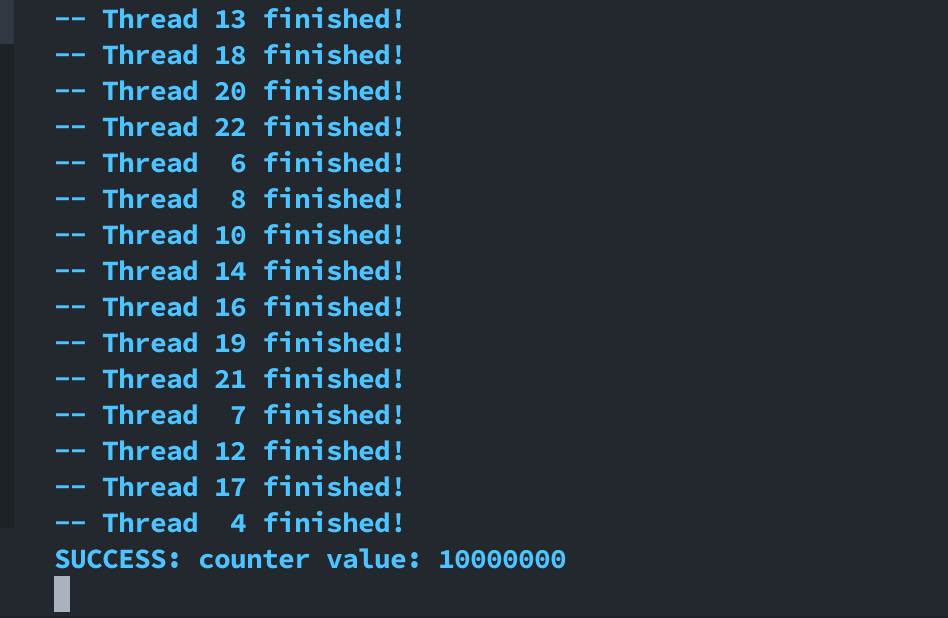
\includegraphics[width=0.8\textwidth]{assets/c3.futex-output.png}
    \caption{Some output from a successful test.}
\end{figure}

\section{Comparing Different Synchronization Methods}

Use the following command to run a test that compares the performance of different
synchronization methods:

\begin{itemize}
    \item With no locks.
    \item With spinlocks.
    \item With mutexes implemented using futex.
\end{itemize}

\begin{verbatim}
    qemu-system-i386 \
        -kernel mos_multiboot.bin \
        -initrd initrd.cpio \
        -serial stdio \
        -append init=/tests/locks-bench
\end{verbatim}

See which method is the fastest, and why?
